% coupling_oil
\begin{figure}[!ht]
\centering
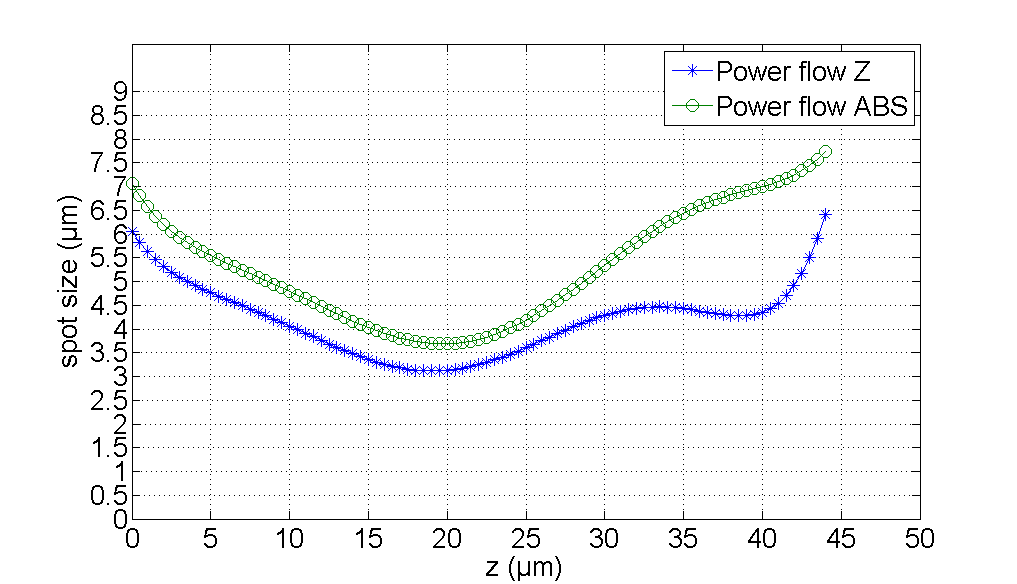
\includegraphics[width=0.7\textwidth]{bilder/spot_curve_oil}
\caption{Spot size curve of TLF in oil.}
\label{fig:oil_spot_curve}
\end{figure}
In default condition the simulation models are surrounded by vacuum background in CST MWS.
In this section we will run the coupling simulation in a different background. For the practical experiment there are not many options for changing the environment. Here the coupling configuration will be placed in an environment full of oil, $n=1.526$ or $\epsilon=2.33$. Changing around conditions of the simulation may greatly affect the working distance of the TLF. Therefore determining the new working distance is necessary before coupling the TLF to the waveguide.  Similar as in section \ref{sect:model_model_model_TLF} the spot size curve Fig. \ref{fig:oil_spot_curve} can be drawn by loading data of TLF beam propagation in oil from CST MWS. Here we can tell from the spot size cure that the minimum spot in oil lies at the position of about $19\mu$m from the TLF, farer than the original minimum spot location in vacuum.\\    

We simulate the coupling setup at the new working distance of $19\mu$m. Fig. \ref{fig:oil_coupling_curve} shows the coupling efficiency in frequency domain of this configuration. The coupling efficiency at working frequency $282$THz achieves about $34.5\%$, which is lower than that of the original configuration in section \ref{sect:model_model_model_TLF}.\\

\begin{figure}[!ht]
\centering
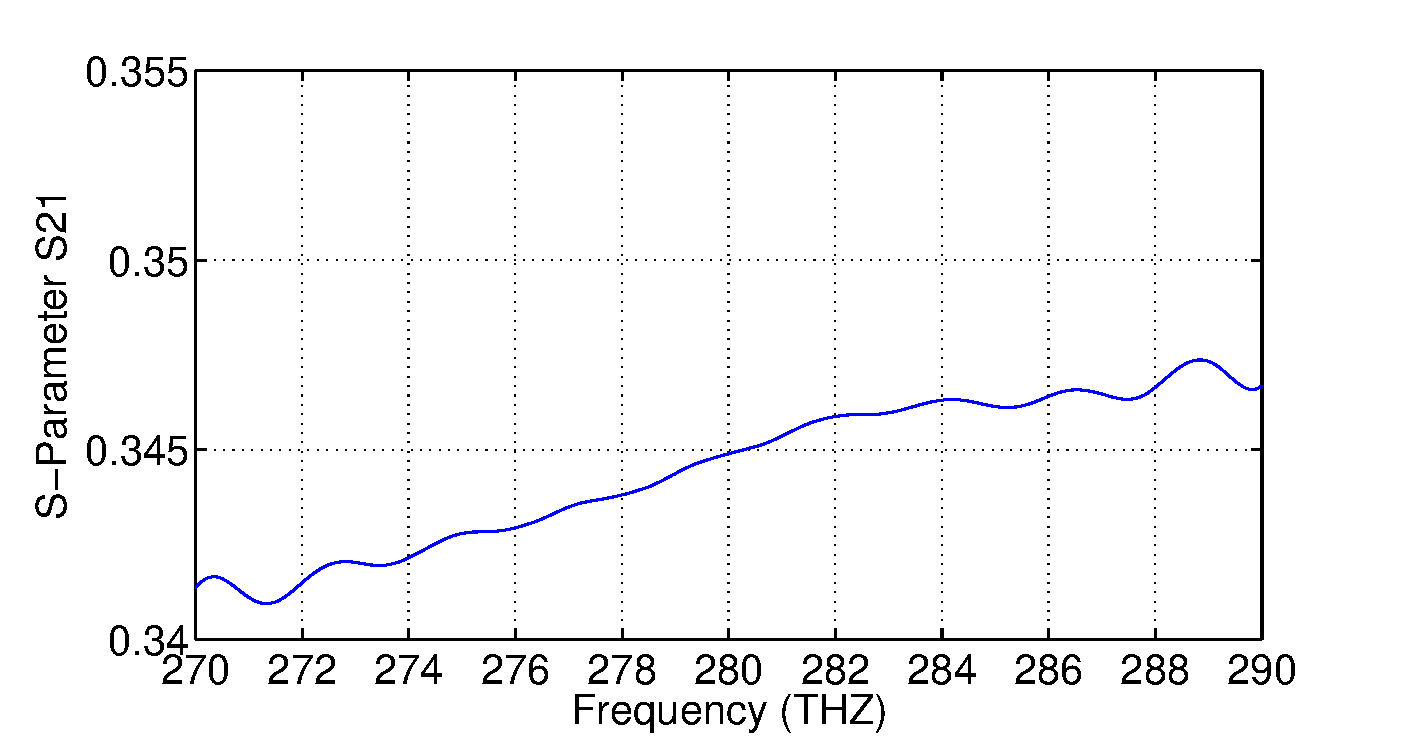
\includegraphics[width=0.7\textwidth]{bilder/s21_oil_curve}
\caption{Coupling efficiency between TLF and the rib waveguide due to frequency domain in oil background.}
\label{fig:oil_coupling_curve}
\end{figure}